\PassOptionsToPackage{expansion=false}{microtype}
\documentclass[sigconf]{acmart}

\usepackage{graphicx}
\usepackage{amsmath}
\usepackage{booktabs}
\usepackage{enumitem}

\settopmatter{printacmref=false}
\renewcommand\footnotetextcopyrightpermission[1]{}
\pagestyle{plain}
\acmConference[ICAIF '26]{ACM ICAIF}{2026}{New York, USA}

\keywords{reinforcement learning, algorithmic collusion, market making, multi-agent systems, market microstructure}

\title{Exchange Rules and Tacit Collusion in a Stylized Reinforcement-Learning Market-Making Game}
\author{Anonymous Author(s)}
\date{}

\begin{document}

\begin{abstract}
That autonomous learning agents can tacitly collude is by now established for price setting and, more recently, for market making: independent reinforcement learning (RL) market makers can learn to sustain supra-competitive spreads without communication. We ask the question that follows and that the emergence literature leaves open, and that has no analog in pricing models because it requires an exchange: which \emph{market-design} levers suppress this collusion? In a stylized repeated spread-setting game we first confirm robust tacit collusion among independent Q-learning market makers (collusion index $\Delta \approx 0.79$ in a duopoly), validated by forced-deviation experiments that exhibit the retaliation-and-reversion dynamics of punishment-supported collusion. We then show that exchange design materially shapes it. A maker rebate, raised toward the half-spread, breaks collusion in the stylized model ($\Delta$ falls from about $0.79$ to $0.11$) and substantially weakens it once a stochastic mid-price and endogenous inventory are added ($0.85$ to $0.48$); in this discrete benchmark structure, coarse tick sizes suppress it while finer grids sustain it; the priority and tie-breaking rule matters; and, as in the pricing literature, collusion erodes with the number of makers, vanishing by four to five competitors. The contribution is diagnostic and design-oriented: in this stylized environment collusion among algorithmic market makers is sensitive to exchange design, identifying levers worth testing in richer market environments.
\end{abstract}

\maketitle

\section{Introduction}

Autonomous algorithms increasingly set prices and quotes in markets. A striking line of work shows that even simple reinforcement learning (RL) agents, optimizing only their own profit with no communication and no instruction to collude, can learn tacitly collusive strategies that sustain supra-competitive prices, enforced by implicit reward and punishment \cite{calvano2020}. This raises an antitrust and market-design concern: collusion can emerge from autonomous learning alone, without any agreement that existing law is equipped to detect.

The same question has been taken to financial market making. Market makers compete by quoting a bid-ask spread; tighter spreads win order flow but earn less per trade, the same volume-margin tension that drives the pricing game. Recent work establishes that the phenomenon carries over to trading: Cont and Xiong \cite{cont2024} analyze the learning dynamics of market-making algorithms in dealer markets and identify the possibility of tacit collusion, and Lillo and Macr\`i \cite{macri2024} document tacit-collusion emergence between two reinforcement-learning agents in a trading game, while one study of multi-agent RL market makers reports competition without collusion in its configuration \cite{wang2025}. The emergence question is therefore largely answered: learning trading agents, including market makers, can collude.

We ask the question that follows, and that the emergence literature, and the pricing-collusion literature entirely, leaves untouched because answering it requires an exchange: \emph{which market-design levers suppress algorithmic collusion?} Tick size, maker-taker rebates, and priority rules are exchange-design choices with no analog in pure price competition, and they are precisely the instruments a venue or regulator can actually set. Our contributions are:
\begin{enumerate}[leftmargin=*]
\item A stylized repeated spread-setting game with elastic order flow, adverse selection, and exchange-design parameters (tick size, maker rebate, tie-breaking rule), with competitive and joint-monopoly benchmarks defining a collusion index $\Delta$ (\S\ref{sec:model}).
\item Confirmation, with rigorous identification, that independent Q-learners collude ($\Delta \approx 0.79$ in a duopoly), validated by forced-deviation experiments exhibiting the retaliation-and-reversion punishment signature (\S\ref{sec:collude}).
\item The core: a controlled comparison of how exchange design affects the \emph{stability} of collusion. A maker rebate raised toward the half-spread breaks it; coarse tick sizes suppress it in the benchmark spread-setting model, although this effect weakens under inventory dynamics; the tie-breaking rule matters; and collusion erodes with the number of makers (\S\ref{sec:conditions}, \S\ref{sec:design}, \S\ref{sec:inventory}). These are concrete, exchange-controlled levers.
\end{enumerate}

The contribution is not a new emergence result. Conditional on tacit collusion being possible, which prior work establishes, we ask whether exchange-design rules make it less stable, and find that several do. We intend this as a clean mechanism study, not a realistic market simulator: the stylization is a deliberate choice that buys well-defined competitive and monopoly benchmarks and interpretable strategies, following the methodology of the algorithmic-pricing literature \cite{calvano2020}, at the cost of institutional realism. The transferable content is the direction of each lever, not the magnitudes, and we make no claim to have solved or quantified algorithmic collusion in real venues. Code, configurations, and random seeds reproducing every figure and table are available.\footnote{Anonymized repository; URL withheld for review.}

\section{Related Work}

\paragraph{Algorithmic collusion.} Calvano et al. \cite{calvano2020} show that independent Q-learning agents in a repeated Bertrand pricing game learn to sustain supra-competitive prices, enforced by punishment, and introduce the collusion index and deviation tests we adopt; Klein \cite{klein2021} studies sequential pricing variants. The concern has reached competition policy \cite{oecd2017,ezrachi2016}, where tacit collusion among autonomous algorithms strains a legal framework built around explicit agreement. In trading, Cont and Xiong \cite{cont2024} analyze the learning dynamics of dealer-market market-making algorithms and identify tacit collusion, and Lillo and Macr\`i \cite{macri2024} document collusion-aligned behavior between two RL agents in an optimal-execution game; Wang et al. \cite{wang2025} study multi-agent RL market makers and report competition without collusion in their configuration. This body of work establishes that collusion can emerge; none studies which exchange-design rules suppress it.

\paragraph{Market design.} The design parameters we vary are classic microstructure policy instruments. Tick size shapes quoting and spreads \cite{harris1994} and has been the subject of regulatory experiments. Maker-taker fee schedules, and the rebates within them, affect liquidity provision and order routing \cite{colliard2012,battalio2016}. Priority and allocation rules are central to limit-order-book design \cite{glosten1994}. This literature studies these levers' effects on liquidity and welfare; we ask, for the first time to our knowledge, how they affect the stability of learned tacit collusion among RL market makers.

\section{A Spread-Setting Market-Making Game}
\label{sec:model}

\paragraph{The game.} $N$ makers play an infinitely repeated game. Each period, maker $i$ simultaneously posts a half-spread $a_i$ from a finite grid $A = \{s_1 < \dots < s_K\}$, quoting bid $-a_i$ and ask $+a_i$ around a mid normalized to zero. Let $a^\star = \min_i a_i$ be the best (tightest) posted spread and $W = \{i : a_i = a^\star\}$ the set of makers posting it. Total two-sided order flow is elastic in the best spread,
\[
Q(a^\star) = q_0\, e^{-\eta\, a^\star},
\]
so tighter quotes draw more volume. Makers in $W$ capture the flow (Bertrand competition) and the rest get nothing. The per-unit margin of a filled maker posting $a$ is
\[
m(a) = a - \mu c + \rho - \kappa,
\]
where $\mu$ is the informed-flow fraction, $c$ the adverse-selection cost per unit, $\rho$ a maker rebate, and $\kappa$ an inventory cost. Per-period profit is
\[
\pi_i =
\begin{cases}
m(a_i)\, Q(a^\star)/|W| & \text{(proportional splitting)},\\
m(a_i)\, Q(a^\star)\,\mathbf{1}[i = w] & \text{(winner-take-all)},
\end{cases}
\]
for $i \in W$ and $\pi_i = 0$ otherwise, where under winner-take-all a single winner $w$ is drawn uniformly from $W$. The exchange-design levers are explicit: the tick size $\delta$ (the spacing of $A$), the maker rebate $\rho$, and the tie-breaking rule. Table~\ref{tab:params} lists all parameters and their default values.

\begin{table}[t]
\caption{Environment and learning parameters (defaults).}
\label{tab:params}
\small
\begin{tabular}{@{}lll@{}}
\toprule
Symbol & Meaning & Default \\
\midrule
$A$ & spread grid & $\{0.1,0.2,0.3,0.4,0.6,0.8,1.0,1.5,2.0\}$ \\
$q_0$ & base order flow & $1.0$ \\
$\eta$ & demand elasticity & $1.0$ \\
$\mu$ & informed-flow fraction & $0.5$ \\
$c$ & adverse-selection cost & $0.2$ \\
$\rho$ & maker rebate & $0.0$ \\
$\kappa$ & inventory cost & $0.0$ \\
tie rule & flow allocation at ties & proportional split \\
\midrule
$\alpha$ & Q-learning rate & $0.125$ \\
$\gamma$ & discount factor & $0.95$ \\
$\varepsilon_t$ & exploration & $e^{-\beta t}$, $\beta=2\times10^{-5}$ \\
$T$ & training periods & $5\times10^{5}$ ($N{=}2$; scaled up for larger $N$) \\
$T_{\text{eval}}$ & evaluation periods & $5\times10^{4}$ (final) \\
seeds & independent runs per cell & $20$ \\
\bottomrule
\end{tabular}
\end{table}

\paragraph{Benchmarks.} Two symmetric outcomes bound behavior and define the collusion index. At the \emph{competitive} (Bertrand) spread $a^N$, makers undercut to the tightest grid spread with strictly positive margin; quoting tighter is the next grid point down, which yields non-positive margin, while quoting wider is undercut. With the defaults $m(a) = a - \mu c = a - 0.1$, so $a^N = 0.2$ (the grid point just above $0.1$), giving per-maker profit $\pi^N = m(0.2)\,Q(0.2)/2 = 0.1\, e^{-0.2}/2 \approx 0.041$. The \emph{joint-monopoly} spread $a^M$ maximizes industry profit $N \cdot m(a)Q(a)/N = m(a)Q(a) = (a-0.1)\,e^{-a}$; the first-order condition $e^{-a}(1.1 - a) = 0$ gives $a = 1.1$, rounded on the grid to $a^M = 1.0$, with $\pi^M = m(1.0)\,Q(1.0)/2 = 0.9\,e^{-1.0}/2 \approx 0.166$. Following \cite{calvano2020} we report the collusion index
\[
\Delta = \frac{\bar\pi - \pi^{N}}{\pi^{M} - \pi^{N}},
\]
where $\bar\pi$ is the realized average per-maker profit over the evaluation window; $\Delta = 0$ is the competitive outcome and $\Delta = 1$ is full collusion. Changing a design lever shifts $a^N$, $a^M$, and the profits, all of which we recompute, so $\Delta$ is comparable across conditions.

\paragraph{Learning.} Each maker is an independent tabular Q-learner with state equal to the previous period's joint action profile (memory one), so the state space has $K^N$ elements and the action space has $K$ spreads. Makers use $\varepsilon$-greedy exploration with $\varepsilon_t = e^{-\beta t}$, learning rate $\alpha$, and discount $\gamma$ (Table~\ref{tab:params}); the Q-update is the standard $Q_i(s,a) \leftarrow Q_i(s,a) + \alpha\,[\,r_i + \gamma \max_{a'} Q_i(s',a') - Q_i(s,a)\,]$. No maker observes another's reward or Q-table and there is no communication. Because $K^N$ grows with $N$, we scale $T$ with the number of makers (to $2.5\times10^6$ at $N{=}4$ and $5\times10^6$ at $N{=}5$). The tabular form keeps strategies interpretable, which the deviation experiments require.

\section{Reinforcement Learners Learn to Collude}
\label{sec:collude}

In a duopoly with adverse selection, independent Q-learners converge to supra-competitive spreads. The competitive benchmark here is a half-spread of $0.2$ and the monopoly spread is $1.0$; the learners settle near a spread of $0.6$, yielding $\Delta \approx 0.79$ (mean over $20$ seeds; Table~\ref{tab:concentration}). The makers therefore recover about four-fifths of the available monopoly markup with no communication.

A high $\Delta$ alone does not establish collusion: two makers might simply coordinate on a focal spread. The decisive test is whether the supra-competitive outcome is \emph{enforced}. We run forced-deviation experiments: after training, makers play greedily until a steady state, then one maker is forced to undercut for a single period, after which all makers resume greedy play. Figure~\ref{fig:punish} shows the result. The deviation triggers immediate retaliation, the non-deviating maker drops its spread toward the competitive level, punishing the deviator, after which both revert to the collusive spread. Quantitatively, in a representative run the collusive spread is $0.6$, the forced undercut is $0.1$, the punisher retaliates to $0.3$, and both revert to $0.6$ within two periods. This retaliation-and-reversion pattern is the reward-punishment signature of tacit collusion \cite{calvano2020}: the supra-competitive spread is sustained by the threat of punishment. A high $\Delta$ without it is not enough; the memoryless variant of \S\ref{sec:conditions} reaches even higher $\Delta$ by coordinating on a focal spread, but cannot punish, so we treat elevated $\Delta$ \emph{and} deviation-induced punishment as jointly necessary for a collusion claim.

\begin{figure}[t]
\centering
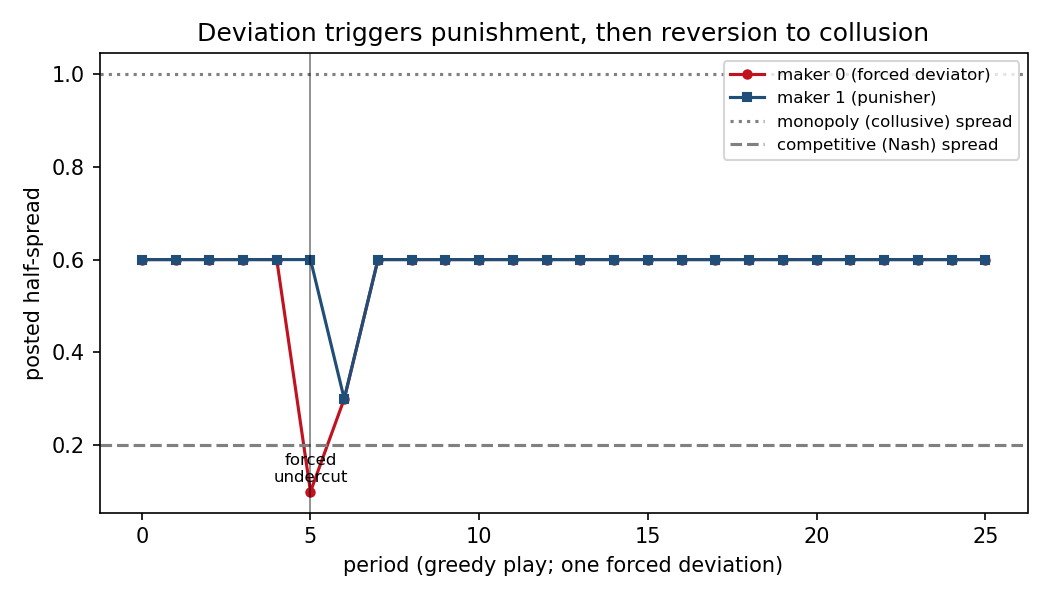
\includegraphics[width=\columnwidth]{results/figure_punishment.png}
\caption{Forced-deviation experiment in a trained duopoly. Both makers sit at the collusive spread; a forced one-period undercut by maker 0 provokes retaliation by maker 1 (a drop toward the competitive spread), followed by reversion to collusion. This punishment dynamic identifies genuine tacit collusion.}
\label{fig:punish}
\end{figure}

\section{Market Structure and Robustness}
\label{sec:conditions}

The duopoly result is not the whole story; collusion is governed by market structure. Figure~\ref{fig:conditions} maps the collusion index across conditions.

\paragraph{Concentration.} Collusion is strongest in a duopoly and erodes monotonically as makers are added: $\Delta$ falls from $0.79$ at $N=2$ to $0.22$ at $N=3$, $0.05$ at $N=4$, and approximately zero by $N=5$ (Table~\ref{tab:concentration}). With enough competitors, Bertrand competition dominates and the learners cannot sustain supra-competitive spreads. This is not an artifact of undertraining the larger state space: doubling the training horizon (to $5\times10^6$ periods at $N=4$ and $10^7$ at $N=5$) leaves $\Delta$ essentially unchanged ($0.03$ and $0.00$ respectively, over $12$ seeds). This directly reconciles our finding with the prior report of competition without collusion \cite{wang2025}: collusion is real but confined to concentrated markets, so a less concentrated configuration sees none.

\paragraph{Collusion is robust to microstructure frictions.} In contrast to concentration, the other conditions do not break collusion (Table~\ref{tab:robust}). Varying the adverse-selection cost from $0$ to $0.6$ leaves $\Delta$ between $0.69$ and $0.87$; varying demand elasticity from $0.5$ to $2.0$ leaves $\Delta$ between $0.64$ and $0.84$, with a mild peak at intermediate elasticity; and varying the exploration decay rate leaves $\Delta$ between $0.69$ and $0.79$. Collusion is likewise insensitive to the learning rate ($\Delta$ between $0.79$ and $0.82$ for $\alpha \in [0.05, 0.2]$). The picture is sharp: tacit collusion among learning market makers is robust to microstructure frictions and learning details but is governed by market concentration.

\paragraph{The role of memory.} The strategic, punishment-supported collusion documented in \S\ref{sec:collude} requires memory: with memory one, the deviation experiment exhibits retaliation. A memoryless (stateless) variant also yields high $\Delta$ ($\approx 0.95$), but there the supra-competitive outcome is coordination on a focal spread that cannot be punishment-enforced, a dynamic known to produce spurious supra-competitive prices in memoryless Q-learning \cite{calvano2020}. We therefore rest the collusion claim on the memory-one case, where the punishment mechanism is directly demonstrated, rather than on profit levels alone.

\begin{figure*}[t]
\centering
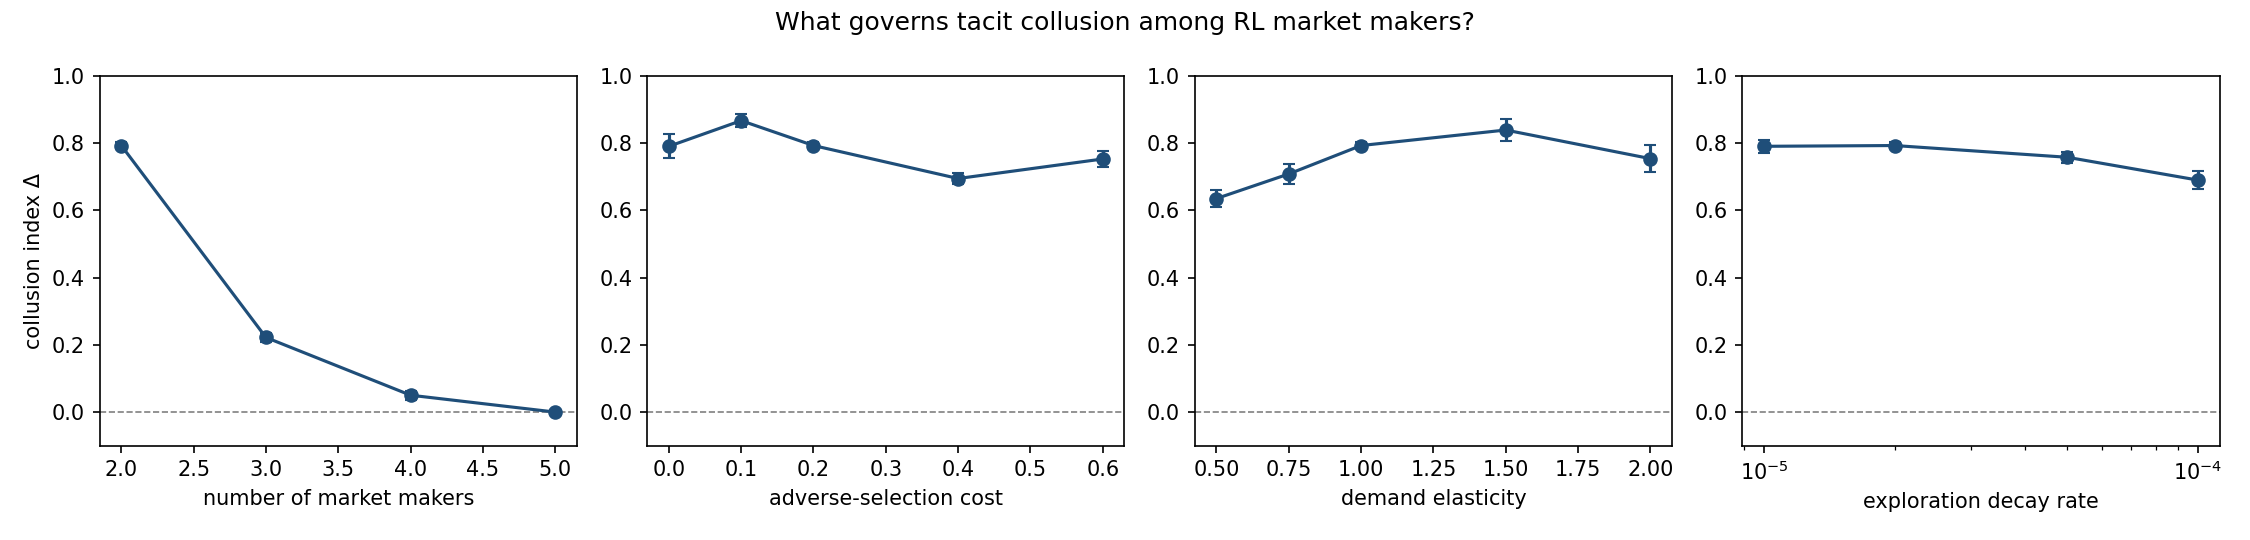
\includegraphics[width=\textwidth]{results/figure_conditions.png}
\caption{Conditions map. The collusion index $\Delta$ as a function of the number of makers, adverse-selection cost, demand elasticity, and exploration rate (means with standard errors over training seeds). Collusion is concentrated in markets with few makers.}
\label{fig:conditions}
\end{figure*}

\section{Exchange Design Shapes Collusion}
\label{sec:design}

Concentration is one lever, but it is largely outside a venue's control. The contribution of this paper is that the exchange's own design choices, which it does control, materially shape whether collusion takes hold. We vary three such choices at the duopoly, holding everything else fixed (Figure~\ref{fig:design}, Table~\ref{tab:design}). Table~\ref{tab:raw} reports the underlying realized spreads and profits alongside the recomputed benchmarks, and a two-sided bootstrap test of each condition's $\Delta$ against the no-rebate baseline. The suppressive effects below (large rebate, coarse tick, winner-take-all) are each significant at $p < 0.001$; the small-rebate increase in $\Delta$ is also significant but at a weaker level ($p = 0.002$ at $\rho = 0.05$). The realized-spread column confirms the effects are behavioral, not benchmark-normalization artifacts.

\paragraph{Rebates reduce collusion in the spread-setting model.} A maker rebate, a per-fill payment to liquidity providers that is standard in maker-taker fee schedules, is the most effective lever we find. A small rebate slightly aids collusion by widening the profit cushion, but as the rebate is raised toward the half-spread it sharply erodes collusion: $\Delta$ falls from $0.79$ with no rebate to $0.52$, $0.29$, and finally $0.11$ as the rebate grows to $0.40$. The mechanism is intuitive: a generous rebate makes tight quoting profitable on its own, so undercutting to capture the rebate-subsidized flow dominates holding the collusive spread, and competition reasserts itself. The fall in $\Delta$ is not a normalization artifact of recomputing the benchmark under the rebate: the realized average half-spread itself falls from $0.63$ at no rebate to $0.15$ at a rebate of $0.40$, a genuine behavioral shift toward tighter quoting (per-maker profit stays roughly constant, $0.14$ to $0.19$). Fee design thus moves quoting behavior, not just the index.

\paragraph{Coarse tick sizes suppress $\Delta$ under the discrete benchmark structure.} Tick size, the granularity of the spread grid, sustains collusion across fine-to-moderate values ($\Delta \approx 0.73$ to $0.81$ for ticks from $0.1$ to $0.3$) but collapses it at coarse ticks ($\Delta = 0.44$ at a tick of $0.4$ and essentially zero at a tick of $0.5$). The mechanism is specific to the structure here: as the grid coarsens, the only spreads near the collusive optimum ($a^M \approx 1.0$) become sparse, and at the coarsest grids the competitive spread $a^N$ and the best collusive option collapse toward the same few levels, so the gap that collusion exploits disappears. We flag that this runs opposite to a common market-microstructure intuition, that wider ticks can \emph{protect} maker rents by blunting undercutting; that intuition concerns a fixed competitive benchmark, whereas here the benchmark and the collusive target move together with the grid. The direction is therefore a property of this discrete benchmark structure and should not be read as a general claim that coarsening ticks reduces collusion in real venues.

\paragraph{Priority rules matter.} The rule for allocating flow when makers post equal tightest spreads also matters. Replacing proportional splitting with winner-take-all, where one maker captures all flow at a tie, lowers $\Delta$ from $0.79$ to $0.67$: when matching the collusive spread no longer guarantees a share, the incentive to undercut strengthens.

\paragraph{Scope of the rebate result.} The rebate finding likewise reflects this environment: a large rebate makes tight quoting profitable on its own, so undercutting to capture rebate-subsidized flow dominates holding the collusive spread. We do not claim that maker rebates reduce collusion in real exchanges, where rebates interact with routing incentives, payment for order flow, and liquidity provision in ways absent here. What the experiments establish is that, within a controlled game, exchange-design parameters move the stability of learned collusion, and in which direction each moves it under these assumptions.

\paragraph{Mechanisms.} The four levers act through a common channel, the temptation to undercut relative to the value of holding the collusive spread. A maker rebate raises the payoff to tight quoting, increasing the undercut temptation. A coarse grid collapses the distance between the competitive and collusive spread choices in this benchmark structure, leaving little room above competition to coordinate on. Winner-take-all lowers the value of matching the collusive spread, since equal quotes no longer guarantee shared flow. And additional makers raise undercutting pressure directly. In each case the design choice shifts the repeated-game incentives that punishment must overcome.

\begin{figure*}[t]
\centering
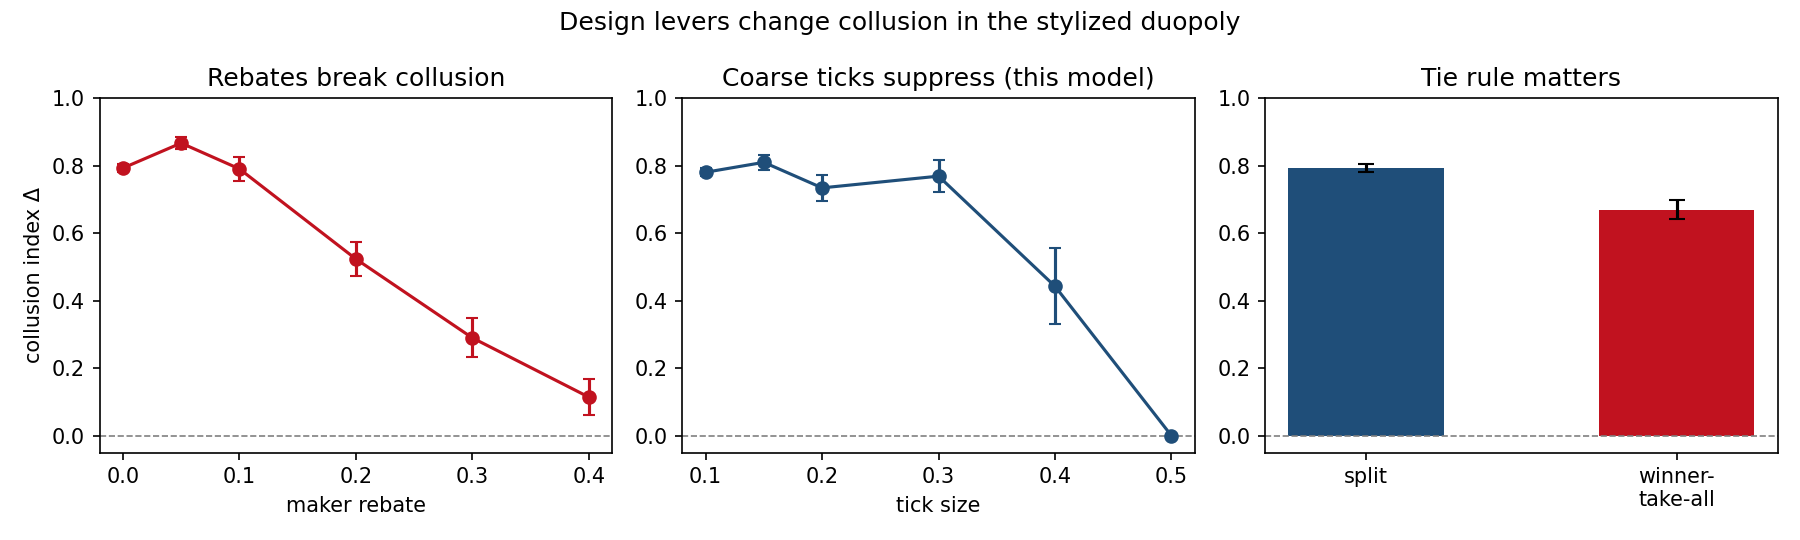
\includegraphics[width=\textwidth]{results/figure_design.png}
\caption{Exchange design shapes collusion in the model (duopoly, means with standard errors over $20$ seeds). A sufficiently large maker rebate breaks collusion; coarse tick sizes suppress it in this discrete benchmark structure (see \S\ref{sec:design}); and winner-take-all tie-breaking weakens it relative to proportional splitting.}
\label{fig:design}
\end{figure*}

\begin{table}[t]
\caption{Collusion vs.\ number of makers (mean $\Delta$, standard error, bootstrap 95\% CI, seeds).}
\label{tab:concentration}
\small
\begin{tabular}{@{}lcccc@{}}
\toprule
$N$ & $\Delta$ & SE & 95\% CI & seeds \\
\midrule
2 & 0.792 & 0.011 & $[0.772,\,0.817]$ & 20 \\
3 & 0.222 & 0.012 & $[0.199,\,0.246]$ & 20 \\
4 & 0.050 & 0.013 & $[0.028,\,0.078]$ & 20 \\
5 & -0.000 & 0.007 & $[-0.012,\,0.012]$ & 20 \\
\bottomrule
\end{tabular}
\end{table}

\begin{table}[t]
\caption{Market-design levers at the duopoly (mean $\Delta$, SE, bootstrap 95\% CI, seeds).}
\label{tab:design}
\small
\begin{tabular}{@{}lcccc@{}}
\toprule
lever value & $\Delta$ & SE & 95\% CI & seeds \\
\midrule
\multicolumn{5}{@{}l}{\emph{Maker rebate} $\rho$}\\
0.00 & 0.792 & 0.011 & $[0.772,\,0.817]$ & 20 \\
0.05 & 0.867 & 0.019 & $[0.830,\,0.902]$ & 20 \\
0.10 & 0.790 & 0.036 & $[0.720,\,0.857]$ & 20 \\
0.20 & 0.523 & 0.051 & $[0.429,\,0.620]$ & 20 \\
0.30 & 0.290 & 0.058 & $[0.176,\,0.397]$ & 20 \\
0.40 & 0.114 & 0.053 & $[0.024,\,0.226]$ & 20 \\
\midrule
\multicolumn{5}{@{}l}{\emph{Tick size} $\delta$}\\
0.10 & 0.780 & 0.012 & $[0.758,\,0.803]$ & 20 \\
0.15 & 0.810 & 0.022 & $[0.769,\,0.850]$ & 20 \\
0.20 & 0.734 & 0.038 & $[0.663,\,0.807]$ & 20 \\
0.30 & 0.769 & 0.048 & $[0.667,\,0.847]$ & 20 \\
0.40 & 0.442 & 0.112 & $[0.245,\,0.640]$ & 20 \\
0.50 & -0.000 & 0.000 & $[-0.000,\,-0.000]$ & 20 \\
\midrule
\multicolumn{5}{@{}l}{\emph{Tie-breaking rule}}\\
split & 0.792 & 0.011 & $[0.772,\,0.817]$ & 20 \\
winner-take-all & 0.669 & 0.029 & $[0.618,\,0.726]$ & 20 \\
\bottomrule
\end{tabular}
\end{table}

\begin{table}[t]
\caption{Robustness at the duopoly: collusion is insensitive to these (mean $\Delta$, SE, 95\% CI, seeds).}
\label{tab:robust}
\small
\begin{tabular}{@{}lcccc@{}}
\toprule
axis value & $\Delta$ & SE & 95\% CI & seeds \\
\midrule
\multicolumn{5}{@{}l}{\emph{Adverse-selection cost} $c$}\\
0.00 & 0.790 & 0.036 & $[0.721,\,0.856]$ & 20 \\
0.10 & 0.867 & 0.019 & $[0.830,\,0.901]$ & 20 \\
0.20 & 0.792 & 0.011 & $[0.772,\,0.817]$ & 20 \\
0.40 & 0.694 & 0.017 & $[0.666,\,0.729]$ & 20 \\
0.60 & 0.753 & 0.024 & $[0.704,\,0.792]$ & 20 \\
\midrule
\multicolumn{5}{@{}l}{\emph{Demand elasticity} $\eta$}\\
0.50 & 0.635 & 0.024 & $[0.592,\,0.684]$ & 20 \\
0.75 & 0.708 & 0.030 & $[0.657,\,0.766]$ & 20 \\
1.00 & 0.792 & 0.011 & $[0.772,\,0.817]$ & 20 \\
1.50 & 0.839 & 0.031 & $[0.775,\,0.895]$ & 20 \\
2.00 & 0.754 & 0.041 & $[0.675,\,0.832]$ & 20 \\
\midrule
\multicolumn{5}{@{}l}{\emph{Exploration decay} $\beta$}\\
1e-05 & 0.790 & 0.019 & $[0.756,\,0.829]$ & 20 \\
2e-05 & 0.792 & 0.011 & $[0.772,\,0.817]$ & 20 \\
5e-05 & 0.758 & 0.016 & $[0.726,\,0.789]$ & 20 \\
1e-04 & 0.690 & 0.028 & $[0.636,\,0.743]$ & 20 \\
\bottomrule
\end{tabular}
\end{table}

\begin{table}[t]
\caption{Raw outcomes and significance for the design levers (duopoly, 20 seeds). $a^N$, $a^M$: competitive and monopoly spreads (recomputed per condition); realized spread and profit are means over seeds; $\Delta$ is the collusion index; $p$ is a two-sided bootstrap test of $\Delta$ against the no-rebate baseline. $^{*}$ marks $p<0.05$.}
\label{tab:raw}
\small
\begin{tabular}{@{}lcccccc@{}}
\toprule
condition & $a^N$ & $a^M$ & spread & profit & $\Delta$ & $p$ \\
\midrule
\multicolumn{7}{@{}l}{\emph{rebate}}\\
$\rho=0.00$ & 0.20 & 1.00 & 0.62 & 0.140 & 0.792 & 0.985 \\
$\rho=0.05$ & 0.10 & 1.00 & 0.70 & 0.154 & 0.867$^{*}$ & 0.002 \\
$\rho=0.10$ & 0.10 & 1.00 & 0.66 & 0.155 & 0.790 & 0.949 \\
$\rho=0.20$ & 0.10 & 1.00 & 0.51 & 0.149 & 0.523$^{*}$ & 0.000 \\
$\rho=0.30$ & 0.10 & 0.80 & 0.29 & 0.161 & 0.290$^{*}$ & 0.000 \\
$\rho=0.40$ & 0.10 & 0.80 & 0.15 & 0.189 & 0.114$^{*}$ & 0.000 \\
\multicolumn{7}{@{}l}{\emph{tick size}}\\
$\delta=0.10$ & 0.20 & 1.10 & 0.79 & 0.139 & 0.780 & 0.426 \\
$\delta=0.15$ & 0.25 & 1.15 & 0.80 & 0.146 & 0.810 & 0.494 \\
$\delta=0.20$ & 0.30 & 1.10 & 0.81 & 0.142 & 0.734 & 0.132 \\
$\delta=0.30$ & 0.40 & 1.00 & 0.82 & 0.151 & 0.769 & 0.660 \\
$\delta=0.40$ & 0.50 & 1.30 & 0.72 & 0.140 & 0.442$^{*}$ & 0.000 \\
$\delta=0.50$ & 0.60 & 1.10 & 0.60 & 0.137 & -0.000$^{*}$ & 0.000 \\
\multicolumn{7}{@{}l}{\emph{tie rule}}\\
split & 0.20 & 1.00 & 0.62 & 0.140 & 0.792 & 0.992 \\
winner-take-all & 0.20 & 1.00 & 0.86 & 0.124 & 0.669$^{*}$ & 0.000 \\
\bottomrule
\end{tabular}
\end{table}


\section{Robustness: A Stochastic Mid-Price and Inventory}
\label{sec:inventory}

The stylized game holds the mid-price fixed and ignores inventory, the two omissions most likely to change the incentive to undercut: a maker that wins the flow accumulates a position that is marked to market against a moving mid and is costly to carry. We therefore re-run the duopoly experiments in an extended game that adds these dynamics and ask whether the headline result and the design levers survive.

In the extended game the mid-price follows a random walk with volatility $\sigma_m = 0.3$; each period the captured flow carries a random buy/sell imbalance, so the winning maker accumulates inventory; inventory is marked to market against the mid move, penalized quadratically ($\kappa = 0.3$), and mean-reverts each period at rate $0.2$ to represent hedging or offload. The learner's state is augmented with the maker's own inventory, discretized into five equal-width signed bins spanning the inventory cap $[-20, 20]$, so quoting can be inventory-dependent; the tabular state space is thus $K^N$ joint-spread profiles times five inventory bins. Spread capture is otherwise unchanged, so the competitive and monopoly benchmarks remain well defined and are recomputed by simulating symmetric play in the extended dynamics. All other settings match the stylized duopoly.

Table~\ref{tab:inventory} compares the two models. Collusion still emerges: the baseline index is $\Delta = 0.85$, slightly above the $0.79$ of the stylized game, so adding inventory risk does not dissolve the supra-competitive coordination, if anything it makes holding a wide collusive spread marginally more attractive than fighting for flow that brings a costly position. The rebate and tie-rule levers act in the same direction as before: a full rebate cuts $\Delta$ to $0.48$ (from $0.85$) and lowers the realized half-spread from $0.75$ to $0.35$, and winner-take-all priority lowers $\Delta$ to $0.76$. The tick-size effect is the one that weakens: a coarse tick of $0.50$ leaves $\Delta = 0.70$ here, versus essentially zero in the stylized model. This is consistent with the caveat in \S\ref{sec:design} that the tick result is a property of the discrete benchmark structure rather than a general force; once the benchmarks are recomputed under the richer dynamics, coarsening the grid no longer collapses the gap that collusion exploits. The two levers we present as the more transferable, fee design and priority, are also the two that survive the added realism.

\begin{table}[t]
\centering
\caption{Collusion index $\Delta$ in the stylized model versus the extended model with a stochastic mid-price and endogenous inventory (duopoly, $20$ seeds each). Collusion still emerges, and the rebate and tie-rule levers move $\Delta$ in the same direction; the tick-size effect weakens, consistent with its dependence on the discrete benchmark structure (\S\ref{sec:design}).}
\label{tab:inventory}
\begin{tabular}{lcc}
\toprule
Condition & $\Delta$ (stylized) & $\Delta$ (mid+inventory) \\
\midrule
No lever (baseline) & 0.79 & 0.85 \\
Maker rebate $\rho=0.40$ & 0.11 & 0.48 \\
Coarse tick $=0.50$ & -0.00 & 0.70 \\
Winner-take-all & 0.67 & 0.76 \\
\bottomrule
\end{tabular}
\end{table}


\section{Discussion}

That independent RL market makers can learn punishment-enforced tacit collusion confirms recent findings \cite{cont2024,macri2024}. Our contribution is what follows: in this controlled environment the behavior is not fixed but is shaped by exchange design. A sufficiently large maker rebate, a coarse tick size, winner-take-all priority, and added competitors each suppress collusion. The results suggest that, in controlled spread-setting environments, collusion is design-sensitive rather than fixed; we read this as identifying levers worth testing in richer settings, not as direct guidance to regulators.

\paragraph{Why a stylized game.} The goal is identification, not realism. A full limit-order-book simulator would add institutional detail but would also make the competitive and monopoly benchmarks, and hence the collusion index, ambiguous: without sharp benchmarks one cannot say by how much behavior is supra-competitive, nor cleanly attribute a change to a design lever. The spread-setting abstraction isolates the question we care about, whether exchange-controlled payoff rules change the learned punishment strategies that sustain collusion, while keeping those benchmarks well defined. We therefore read the magnitudes as model-specific and the directions as the transferable content.

\paragraph{Limitations.} A stochastic mid-price and endogenous inventory, the two omissions most likely to alter the undercutting incentive, are tested directly in \S\ref{sec:inventory}: collusion persists and the rebate and priority levers act in the same direction, while the tick-size effect weakens as its benchmark-structure dependence predicts. The model still omits much of real market making, and each remaining omission is a natural extension rather than a hidden assumption: asymmetric makers (heterogeneous costs, rebates, or risk), latency and queue position, order cancellation and re-quoting, order routing across venues, and multi-asset effects. On the learning side, we use tabular Q-learning with memory one; deep function approximation and richer memory are the obvious next steps. These choices buy clean benchmarks and interpretable strategies at the cost of realism, and the quantitative results should be read in that light.

\section{Conclusion}

Reinforcement learning market makers in this stylized game learn to tacitly collude on supra-competitive spreads, with no communication, enforced by retaliation. More usefully, the behavior is a function of exchange design: maker rebates, tick size, priority rules, and the number of competitors each shape it, and several break collusion outright in the model. In this stylized environment, then, tacit collusion among RL market makers is not fixed but is sensitive to exchange-design parameters. Establishing the same levers under richer learning and in full order-book environments is the natural next step.

\bibliographystyle{ACM-Reference-Format}
\bibliography{collusion_refs}

\end{document}
